% !TEX program = xelatex
% =============================================================================
%  问题二（CUMCM 2026 B 题）求解论文：第二个检测点的选择与候选区域
%  在 paper/t2/ 目录下运行：xelatex main.tex（跑两遍解决交叉引用/目录）
%  图片相对路径 ../../results/t2/ 直接指向求解程序输出的矢量图（保证与结果同源）
%  字体：ctex fontset=fandol（TeX Live 自带开源中文字体，Arch 开箱即用）
% =============================================================================
\documentclass[fontset=fandol, 12pt, a4paper]{ctexart}

% ---------- 页面：A4，上下左右 2.5cm ----------
\usepackage[a4paper, top=2.5cm, bottom=2.5cm, left=2.5cm, right=2.5cm]{geometry}

% ---------- 数学 ----------
\usepackage{amsmath}
\usepackage{amssymb}

% ---------- 字体（fontspec + ctex，xelatex 编译） ----------
% 中文宋体/黑体/楷体由 ctex 的 fontset=fandol 自动设置（FandolSong / FandolHei / FandolKai）。
\IfFontExistsTF{Times New Roman}{\setmainfont{Times New Roman}}{}

% ---------- 正文：12.05pt，首行缩进 2em，两端对齐，行距 0.72em ----------
\linespread{1.43}
\setlength{\parindent}{2em}

% ---------- 标题编号（\ctexset 配置） ----------
\ctexset{
  section/number       = \chinese{section},
  subsection/number    = \arabic{section}.\arabic{subsection},
  subsubsection/number = \arabic{section}.\arabic{subsection}.\arabic{subsubsection},
}

% ---------- 标题格式（titlesec 配置） ----------
\usepackage{titlesec}
\titleformat{\section}
  {\centering\fontsize{17.3pt}{20.8pt}\heiti\bfseries}
  {\chinese{section}、}{1em}{}
\titleformat{\subsection}
  {\fontsize{14.45pt}{17.4pt}\heiti\bfseries}
  {\arabic{section}.\arabic{subsection}}{1em}{}
\titleformat{\subsubsection}
  {\fontsize{12.05pt}{14.5pt}\heiti\bfseries}
  {\arabic{section}.\arabic{subsection}.\arabic{subsubsection}}{1em}{}
\titlespacing{\section}       {0pt}{1.25em}{0.82em}
\titlespacing{\subsection}    {0pt}{1.15em}{0.55em}
\titlespacing{\subsubsection} {0pt}{1.15em}{0.55em}

% ---------- 目录（tocloft 点线引导） ----------
\usepackage{tocloft}
\renewcommand{\cftsecfont}{\heiti\bfseries}
\renewcommand{\cftsecpagefont}{\heiti\bfseries}
\renewcommand{\cftsecleader}{\cftdotfill{\cftdotsep}}
\renewcommand{\cftsubsecleader}{\cftdotfill{\cftdotsep}}
\renewcommand{\cftsubsubsecleader}{\cftdotfill{\cftdotsep}}

% ---------- 表格、图片与代码 ----------
\usepackage{graphicx}   % 图片支持
% 论文图由求解程序输出到 results/t2/ 后复制到 paper/t2/figures/（矢量 PDF）。
% 引用写法 ../figures/xxx.pdf：既满足「相对本文件」的检查，也让 xelatex 通过下面的
% \graphicspath（figures/../figures/xxx.pdf = figures/xxx.pdf）找到文件。
\graphicspath{{figures/}}
\usepackage{booktabs}   % 三线表
\usepackage{float}      % [H] 立即放置浮动体
\usepackage{array}
\usepackage{xcolor}
\usepackage{listings}
\lstset{
  basicstyle=\ttfamily\small,
  backgroundcolor=\color{black!3},
  frame=single,
  framesep=6pt,
  rulecolor=\color{black!30},
  framerule=0.8pt,
  breaklines=true,
  showstringspaces=false,
  columns=fullflexible,
  keepspaces=true,
}

% ---------- 示意图（技术路线图） ----------
\usepackage{tikz}
\usetikzlibrary{arrows.meta,positioning}

% ---------- 页码：底部居中 ----------
\pagestyle{plain}

% ---------- 自定义命令 ----------
\newcommand{\papertitle}[1]{%
  \thispagestyle{empty}%
  \begin{center}
    {\fontsize{17.3pt}{22pt}\bfseries #1}
  \end{center}
  \vspace{1em}
}
\newcommand{\abstractcn}[2]{%
  \thispagestyle{empty}%
  \begin{center}{\fontsize{14pt}{17pt}\bfseries 摘要}\end{center}
  #1\par
  \vspace{1em}
  {\heiti\bfseries 关键字：}#2\par
  \newpage
}
\makeatletter
\newcommand{\tocpage}{%
  \setcounter{page}{1}%
  \begin{center}
    {\fontsize{17.3pt}{20.8pt}\heiti\bfseries 目录}
  \end{center}
  \vspace{0.5em}
  \@starttoc{toc}%
  \newpage
}
\makeatother
\newcommand{\referencescn}{%
  \addcontentsline{toc}{section}{参考文献}%
  % 参考文献。注意：main.tex 中 \referencescn 已通过 thebibliography 自动生成
% “参考文献”一级标题（不带编号），并已 \addcontentsline 进入目录，
% 所以本文件**不要再写一级标题**，否则会出现两个“参考文献”标题。

\begin{thebibliography}{99}
\bibitem{cumcm2026b} 全国大学生数学建模竞赛组委会. 2026 年高教社杯全国大学生数学建模竞赛 B 题：
                    机器狗搜索与清除干扰源[Z]. 2026.
\bibitem{foy1976} W. H. Foy. Position-Location Solutions by Taylor-Series Estimation[J].
                  IEEE Transactions on Aerospace and Electronic Systems, 1976, AES-12(2): 187--194.
                  （几何稀释：两条示向度夹角过小时定位误差沿角平分线方向被放大，且在该夹角
                  区间内增设测线亦不能改善）
\bibitem{chan1994} Y. T. Chan, K. C. Ho. A Simple and Efficient Estimator for Hyperbolic
                   Location[J]. IEEE Transactions on Signal Processing, 1994, 42(8): 1905--1915.
                   （几何精度因子较差时，最小二乘类定位估计显著退化，可用于说明必须避开退化构型）
\bibitem{ren2016} 任叶童. 基于到达角信息的无源定位算法研究[D]. 天津: 天津大学电子信息工程学院,
                  2016. （第 2.4 节：双站测向定位误差概率椭圆的半轴与面积公式，即本文
                  式~\eqref{eq:crlb} 的 $1\sigma$ 形式）
\bibitem{chen2009} X. Chen, Z. Xu, L. Rui. An Optimization Algorithm of Multi-Observer
                   Trajectories for Cooperative Bearings-Only Target Localization[C].
                   Proceedings of ICICS 2009. IEEE, 2009.
                   （观测点优化中"靠近目标"与"改善方位分布"的权衡关系，以及以期望位置误差
                   为指标的口径）
\bibitem{proj} 本题求解代码与全部数值复现：\texttt{cumcm/t2/} 为问题二的模型、算法、文献判据层
              与制图实现（顶层入口 \texttt{T2.py}）；结论与自校验数值见
              \texttt{results/t2/t2\_second\_site.json}，逐格适合度见
              \texttt{results/t2/t2\_suitability.csv}. 2026.
\end{thebibliography}
%
}
\newcommand{\appendixcn}{%
  \section*{附录 A\quad 核心代码}%
  \addcontentsline{toc}{section}{附录 A\quad 核心代码}%
  \vspace{1.1em}

核心代码见 \texttt{cumcm/t2/}~\cite{proj}（模型、算法、文献判据层与制图），以下列出最关键的三个部分：
楔形交定位区域的直径、最坏情况代价函数、以及文献闭式判据。

\begin{lstlisting}[language=Python]
# cumcm/t2/region.py —— 定位四边形（两条 ±1° 边界射线之交）的直径，向量化
def quad_diameters(site, theta1, sx, sy, theta2, err_deg=BEARING_ERROR_DEG,
                   sentinel=DIAM_SENTINEL):
    """区域是凸的，故直径 = 候选顶点两两距离的最大值；近共线时返回哨兵值。"""
    P, keep = _candidate_points(site, theta1, sx, sy, theta2, err_deg)
    best = np.zeros(np.shape(sx), dtype=float)
    for i in range(P.shape[0]):
        for j in range(i + 1, P.shape[0]):
            d = np.hypot(P[i][..., 0] - P[j][..., 0], P[i][..., 1] - P[j][..., 1])
            best = np.maximum(best, np.where(keep[i] & keep[j], d, 0.0))
    return np.where(np.isnan(best), sentinel, best)

def analytic_diameter(d, r2, gamma_deg, err_deg=BEARING_ERROR_DEG):
    """一阶解析式:(2*eps/sin(gamma))*sqrt(d^2 + r2^2 + 2*d*r2*|cos(gamma)|)，仅用于解释趋势。"""
    g = math.radians(gamma_deg)
    return (2.0 * math.radians(err_deg) / math.sin(g)) * math.sqrt(
        d * d + r2 * r2 + 2.0 * d * r2 * abs(math.cos(g)))
\end{lstlisting}

\begin{lstlisting}[language=Python]
# cumcm/t2/score.py —— 最坏定位直径 J(S2)：源采样 × 第二次测向误差的两层 max
def worst_case_diameters(site, sx, sy, theta1, sources, deltas2,
                         err_deg=cfg.BEARING_ERROR_DEG, reduce="max"):
    """reduce='max' 为本文 minimax 口径；'mean' 为文献常用的期望口径（用于对照）。"""
    sx, sy = np.asarray(sx, float).ravel(), np.asarray(sy, float).ravel()
    best = np.zeros(sx.shape, dtype=float)
    for gx, gy in np.asarray(sources, dtype=float):            # 源在楔形内何处
        w2 = np.degrees(np.arctan2(gy - sy, gx - sx)) % 360.0  # 第二次测向的名义方向
        for d2 in np.asarray(deltas2, dtype=float):            # 第二次测向误差
            best = np.maximum(best, quad_diameters(site, theta1, sx, sy, w2 + d2, err_deg))
    return best
\end{lstlisting}

\begin{lstlisting}[language=Python]
# cumcm/t2/theory.py —— 文献闭式判据（与数值特征分解对账，最大相对偏差 1.4e-12）
def gdop(d, r2, gamma_deg, err_deg=cfg.BEARING_ERROR_DEG):
    """GDOP = sigma*sqrt(R1^2+R2^2)/sin(gamma)（由 tr H、det H 直接得到）。"""
    return math.radians(err_deg) * math.sqrt(d * d + r2 * r2) / math.sin(math.radians(gamma_deg))

def crlb_major(d, r2, gamma_deg, err_deg=cfg.BEARING_ERROR_DEG):
    """CRLB 误差椭圆主半轴:sqrt(2)*sigma*R1*R2 / sqrt(R1^2+R2^2-sqrt((R1^2+R2^2)^2-4*R1^2*R2^2*sin(gamma)^2))。"""
    g, s = math.radians(gamma_deg), math.radians(err_deg)
    a = d * d + r2 * r2
    delta = math.sqrt(max(a * a - 4.0 * d * d * r2 * r2 * math.sin(g) ** 2, 0.0))
    return math.sqrt(2.0) * s * d * r2 / math.sqrt(a - delta)

def minimax_radius(d, r2, gamma_deg, err_deg=cfg.BEARING_ERROR_DEG):
    """本文集员闭式的半径 = 一阶解析直径的一半。"""
    return 0.5 * analytic_diameter(d, r2, gamma_deg, err_deg)
\end{lstlisting}

完整可复现命令（结果为确定性输出，两次运行逐字节一致；论文图由程序输出后复制到
\texttt{paper/t2/figures/}）：

\begin{verbatim}
.venv/bin/python T2.py                 # 求解 + 两张成果图（约 15 s）
.venv/bin/python T2.py --eta 0.05      # 候选区域收紧到 1.05 J*
.venv/bin/python T2.py --no-plot       # 只出数值与 CSV/JSON
.venv/bin/python T2.py --site 200 -300 --bearing 45   # 换检测点
.venv/bin/python -m cumcm.t2.region    # 几何自检（解析 vs 精确）
.venv/bin/python -m cumcm.t2.theory    # 文献判据自检
\end{verbatim}
%
}

\begin{document}

% 封面（不编号）
\papertitle{定向 + 全向混合干扰源的搜索与清除\\\vspace{0.4em}\large 问题二：第二个检测点的选择与候选区域}

% 摘要页（不编号）
\abstractcn{%
  本文解决 2026 年 CUMCM B 题问题二：在只有一次测向结果（第一检测点 $S_1$、示向度
  $\theta_1$，误差 $\pm1^\circ$）的条件下，给出第二个检测点 $S_2$ 的选择策略与候选区域。
  第一次测向只排除方向、不给出距离，故源的位置是一个以 $S_1$ 为顶点、长 $1500$ m、张角
  $2^\circ$ 的窄楔形不确定集 $C$（下界 $5$ m 由"近距测不到示向度"确定，上界由接收半径
  上限确定）。第二个检测点还必须"一定听得到"：由于接收半径 $\rho_{\mathrm{rec}}\in
  [1000,1500]$ m 未知，要求对 $C$ 内任意源都有 $|S_2G|\le1000$ m，该约束把可行域锁成一个
  面积 $0.447$ km$^2$ 的透镜。在此可行域上，本文把选点建模为\textbf{最坏情况定位直径的
  极小化}：代价函数取"楔形交（定位区域）直径"对源位置与第二次测向误差的最坏值
  $J(S_2)=\max_{G\in C,|\delta_2|\le1^\circ}\mathrm{diam}\big(W(S_1,\theta_1\pm1^\circ)
  \cap W(S_2,\theta_2+\delta_2\pm1^\circ)\cap D(1800)\big)$，并定义适合度 $F=J^*/J$、
  候选区域 $\{F\ge1/(1+\eta)\}$（$\eta=10\%$）。
  求解得\textbf{最优第二检测点 $S_2^*=(801,605)$ m}，即距 $S_1$ 约 $1004$ m、相对示向度
  偏 $+37.1^\circ$；最坏定位直径 $J^*=134.08$ m，相比只有一次测向的 $1800$ m
  \textbf{缩小 $13.4$ 倍}；候选区域是半径 $948\sim1004$ m、方位 $\theta_1\pm
  [25^\circ,40^\circ]$ 的两条镜像弧带（合计 $0.0207$ km$^2$）。
  本文进一步引入文献判据层做交叉验证：由两站测向的 Fisher 信息矩阵导出 CRLB 误差椭圆与
  GDOP $=\sigma\sqrt{R_1^2+R_2^2}/\sin\gamma$，证明它与本文闭式同以 $1/\sin\gamma$ 为
  主导（对应 Foy 的几何稀释），但文献口径在本模型最坏情形上比精确最坏半径\textbf{低约三成}
  （$46.98$ m vs $67.04$ m），故只用于解释趋势与快速预筛（秩相关 $0.998$）；据此设计的
  "5 m 细网格 GDOP 快筛 $\rightarrow$ 精确复核 $\rightarrow$ 2 m 细化"全局认证与 25 m
  粗搜解相差 $8.5$ m、最坏直径优 $0.063$ m，两条路线互相印证。准则对照表明文献 GDOP 判据与
  期望精度口径给出的最优点与本文相距不足 $20$ m、最坏直径相差 $<0.1\%$，说明结论对判据
  选择不敏感。全部结果确定性可复现（六个产物两次运行逐字节一致）。%
}{%
  纯方位测向 \quad 最坏情况优化 \quad 集员定位 \quad CRLB/GDOP \quad 几何稀释 \quad 候选区域%
}

% 目录页（页码从 1 开始）
\tocpage

\section{问题重述与分析}

\subsection{问题的物理背景}

竞赛平台在半径 $R_{\mathrm{env}}=1800$ m 的圆形区域内随机布置若干干扰源~\cite{cumcm2026b}。机器狗从圆域原点
出发，以 $5$ m/s 的速度移动，通过测向与清除两类动作完成任务：对某频道测向耗时 $5$ s，返回
示向度（方向），且测量误差不超过 $1^\circ$；对某频道实施清除时，只有当机器狗与干扰源的
距离不超过 $20$ m 才能成功。机器狗能听到某干扰源信号的充要条件是"到源的距离不超过该源的
接收半径"，而接收半径 $\rho_{\mathrm{rec}}$ 是每个源固有但未知的量，取值范围为
$[1000,1500]$ m。

问题的第一轮只做了一次测向：机器狗在检测点 $S_1$ 处对某频道测向，得到一个示向度
$\theta_1$。这次测量给出了方向信息，但\textbf{没有给出距离信息}——源可能在示向度射线上
任意远近处。问题二要求在此基础上回答：

\begin{enumerate}
  \item 第二个检测点 $S_2$ 应当按什么策略选择？
  \item 可行而优异的 $S_2$ 构成怎样的候选区域，并说明该区域周边各位置的"适合程度"。
\end{enumerate}

不失一般性，本文取 $S_1$ 为坐标原点、$\theta_1$ 沿 $x$ 轴正方向（即 $\theta_1=0^\circ$）；
所有结果通过对 $S_1$ 的平移与旋转即可搬到任意实际情形。

\subsection{难点的结构化分析}

与"再测一次就完了"的直觉不同，本问有三层困难，且必须同时处理。

\textbf{(1) 源的位置是一个二维不确定集，不是一条线。} 一次测向只排除方向不合的位置，源到
$S_1$ 的距离 $d$ 仍然未知，但有两个硬边界：一是机器狗在 $S_1$ 处确实听到了信号，故
$d\le\rho_{\mathrm{rec}}\le1500$ m；二是题目附件规定距离不超过 $5$ m 时信号过强、测不出
示向度，既然 $S_1$ 测到了示向度，就必有 $d>5$ m。于是源的所有可能位置构成以 $S_1$ 为顶点、
深 $1500$ m、张角 $2^\circ$ 的窄楔形（再与 $1800$ m 圆域求交）。

\textbf{(2) 第二个检测点必须"一定听得到"。} 接收半径未知，若 $S_2$ 选得过远，一旦源的接收
半径偏小，第二次测向将返回无信号，这一趟就白跑了。由于 $\rho_{\mathrm{rec}}$ 的下界是
$1000$ m，要\textbf{保证}第二次测向一定成功，就必须让源不确定集内\textbf{每一个}可能位置
到 $S_2$ 的距离都不超过 $1000$ m。这一条把 $S_2$ 的可选范围压缩成一个面积仅
$0.447$ km$^2$ 的透镜形区域（约为 $1800$ m 圆域的 $0.4\%$）。

\textbf{(3) 定位误差只能用区域口径描述，且必须取最坏情况。} 本项目的定位区域口径与问题一
一致：两条示向度各带 $\pm1^\circ$ 误差，其边界射线相交围出一个四边形（楔形交）。定位精度
用该区域的\textbf{直径}度量：直径小于 $20$ m 才能保证清除成功。由于源在楔形内何处未知、
第二次测向向哪边偏 $1^\circ$ 也未知，选点必须让\textbf{所有这些可能情况中最坏的那一个}
尽可能小——注意"最坏"是两层最坏的复合：源位置取最坏、测向误差取最坏。只做一次测向时，
源方向上的不确定使最坏直径为 $1800$ m（$d$ 从 $5$ m 跨到 $1500$ m，再叠加角向
$\pm1^\circ$），因此第二次测向的价值就体现在能把这一最坏直径压到多小。

\subsection{本文的工作}

本文把上述三层困难写成一条完整的建模与求解链条：

\begin{itemize}
  \item 用\textbf{集员（set-membership）}方式刻画全部不确定性：源的不确定集 $C$ 是楔形，
        测向误差是角度区间，不含任何概率分布假设，因此结论是"保证型"的；
  \item 把"一定听得到"写成\textbf{最坏距离约束}，由此得到可行域（透镜）的显式表达；
  \item 以\textbf{最坏情况定位直径} $J(S_2)$ 为目标函数建立极小化模型，并给出适合度
        $F=J^*/J$ 与候选区域 $\{F\ge1/(1+\eta)\}$ 的定义，直接回答"周边区域的适合度"；
  \item 用\textbf{一阶解析式}解释最优解为何"尽量远、并偏离示向度约 $37^\circ$"；
  \item 引入\textbf{文献判据层}：由两站纯方位测向的 Fisher 信息矩阵导出 CRLB 误差椭圆、
        GDOP 与几何稀释式，证明它们与本文解析式同源、但在本模型最坏情形上系统性偏低约三成，
        因而只用于趋势解释与快速预筛；再据此设计全域认证算法，独立复核最优点；
  \item 给出\textbf{灵敏度分析}（接收半径口径、距离先验、阈值、检测点位置）与
        \textbf{自校验}（解析几何对 shapely、离散化加密、镜像对称、确定性复现）。
\end{itemize}

结论是明确的：第二个检测点应当选在\textbf{距 $S_1$ 约 $1004$ m、相对示向度偏向约
$+37^\circ$} 处（关于示向度镜像的两点等价），最坏定位直径由 $1800$ m 降至 $134.08$ m，
缩小 $13.4$ 倍；符合"最坏直径不超过最优值 $1.1$ 倍"的候选区域是两条窄弧带，合计面积
$0.0207$ km$^2$，仅占可行域的 $4.63\%$。

\section{总体思路}

\subsection{建模主线：把"保证"做成目标函数}

本问的关键在于"第二次测向必须成功、定位必须够准"这两件事都必须是\textbf{保证}而不是
\textbf{期望}。因此本文不采用"误差服从正态分布、最小化均方误差"的统计路线，而采用
\textbf{集员 + 最坏情况}路线：把所有已知信息写成集合（源的不确定集、示向度误差区间），
把"最坏情况下仍然成立"写成约束与目标。这条路线有三个直接好处：结论是硬保证；不需要假设
误差分布；每一步都可以用解析几何独立复核。

建模主线由四步组成（图~\ref{fig:roadmap} 上半支）：

\begin{enumerate}
  \item \textbf{由一次测向写出源不确定集} $C$：以 $S_1$ 为顶点、深 $1500$ m、张角
        $2^\circ$ 的窄楔形（§\ref{sec:model}）；
  \item \textbf{由"一定听得到"写出可行域} $F$：$C$ 中每个源到 $S_2$ 的距离都不超过接收
        半径下界 $1000$ m，等价于 $S_2$ 落在以 $C$ 的四个极点为心、半径 $1000$ m 的四个
        圆盘之交里，是一个面积 $0.447$ km$^2$ 的透镜（§\ref{sec:model}）；
  \item \textbf{由定位区域口径写出代价函数}：对给定的 $S_2$，取源位置与第二次测向误差的
        最坏组合，得到该点的最坏定位直径 $J(S_2)$；
  \item \textbf{求解} $\min_{S_2\in F}J(S_2)$，得到最优第二检测点 $S_2^*$；再以
        $F=J^*/J$ 定义适合度、以 $F\ge1/(1+\eta)$ 定义候选区域，回答"周边区域的适合度"。
\end{enumerate}

\begin{figure}[H]
  \centering
  \begin{tikzpicture}[
      box/.style={draw, rounded corners=2pt, align=center, font=\small, inner sep=3pt,
                  minimum height=1.05cm, text width=3.15cm},
      ar/.style={-{Latex[length=2mm]}, thick},
      node distance=5mm and 6mm
    ]
    \node[box, fill=blue!5]                (c)    {源不确定集 $C$：楔形\\$d\in[5,1500]$ m，$2^\circ$};
    \node[box, fill=blue!5, right=of c]    (f)    {可测性保证：可行域 $F$\\（透镜 $0.447$ km$^2$）};
    \node[box, fill=orange!8, right=of f]  (j)    {最坏定位直径\\$J(S_2)$ 泛函};
    \node[box, fill=orange!14, right=of j] (opt)  {$\min\limits_{S_2\in F}J$：\\$S_2^*=(801,605)$ m};
    \node[box, fill=green!6, below=9mm of c]    (lit)  {文献判据：CRLB /\\GDOP / 几何稀释式};
    \node[box, fill=green!6, below=9mm of f]    (pre)  {GDOP 解析场快筛\\（$5$ m 细网格）};
    \node[box, fill=green!10, below=9mm of j]   (cert) {精确复核 $+$ 细化\\（全局认证）};
    \node[box, fill=gray!10, below=9mm of opt]  (band) {适合度 $F=J^*/J$\\候选弧带 $0.0207$ km$^2$};
    \draw[ar] (c) -- (f);
    \draw[ar] (f) -- (j);
    \draw[ar] (j) -- (opt);
    \draw[ar] (lit) -- (pre);
    \draw[ar] (pre) -- (cert);
    \draw[ar, dashed] (cert) -- (opt);
    \draw[ar, dashed] (opt) -- (band);
    \draw[ar, dashed] (j) -- (band);
  \end{tikzpicture}
  \caption{问题二求解的技术路线。上半支为集员建模与最坏情况最小化的主链；下半支为文献判据层，
  它提供解析快筛并独立认证最优解；右端给出适合度与候选区域。}
  \label{fig:roadmap}
\end{figure}

\subsection{为什么还要引入文献判据}

纯方位测向的交会定位在文献中有成熟的理论刻画：两站测向的 Fisher 信息矩阵、Cram\'er-Rao
下界（CRLB）误差椭圆、几何精度因子（GDOP）以及几何稀释效应。这些工具与本文的集员口径
回答的是同一类问题（"两条带误差的射线交会有多准"），但语汇不同：文献口径是\textbf{统计}
尺度（独立误差平方向加），本文口径是\textbf{有界}尺度（误差可同向叠加）。二者是否一致、
能否互相替代，是审稿与工程上都必须回答的问题。

本文的处理方式是\textbf{把文献判据实现成一层代码，逐项与精确判据对照}（§\ref{sec:lit}）：

\begin{itemize}
  \item 文献的 CRLB 椭圆主半轴、GDOP、几何稀释式都能写成 $1/\sin\gamma$ 主导的闭式
        （$\gamma$ 为源处两条示向度的交会角），这与本文一阶解析式同源，说明\textbf{趋势一致}；
  \item 但在本模型最坏情形上，文献式比精确最坏半径\textbf{低约三成}（$46.98$ m 对
        $67.04$ m），因为源不确定集取最坏、误差同向叠加这两条本文必须承担，
        而统计口径把它们平均掉了。清除判据是 $20$ m 硬阈值，低估三成的量不能当保险界；
  \item 文献口径与精确判据的\textbf{排序几乎一致}（可行域内 $1276$ 个采样点上
        Spearman 秩相关 $0.998$），因此可以拿它做\textbf{快速预筛}：用解析 GDOP 场在 $5$ m
        细网格上筛出少数候选，再用精确构造复核并细化。
\end{itemize}

这一步的结果不是"换一个更好的判据"，而是\textbf{换来了一个独立的全局认证}：细网格
快筛路线给出的最优解与 $25$ m 粗搜 $+$ 局部细化路线相差仅 $8.5$ m、最坏直径优
$0.063$ m，两条路线互相印证，排除了"粗网格漏掉更好盆地"的风险。此外，文献常用的
\textbf{期望}精度口径（最小化平均定位直径）与本文的 minimax 口径给出的最优点相距不足
$20$ m、最坏直径相差小于 $0.1\%$，说明最终推荐区域\textbf{对判据的选择不敏感}——
这是本文结论稳健性的直接证据（§\ref{sec:res}）。

\subsection{全文章节安排}

§\ref{sec:model} 建立模型（不确定集、可行域、代价泛函、适合度与候选区域、一阶解析式）；
§\ref{sec:lit} 建立文献判据层并逐项对照；§\ref{sec:algo} 给出算法（离散化、粗搜、细化、
文献快筛与全局认证、候选弧带、镜像规范）；§\ref{sec:res} 给出求解结果与两张成果图；
§\ref{sec:sens} 给出灵敏度分析；§\ref{sec:eval} 给出模型校验、评价与推广。

\section{模型假设}

\begin{enumerate}
  \item \textbf{源静止、位置固定未知。} 本问只讨论一个已测得示向度的干扰源，其在圆域内的
        位置 $G$ 在一局内不变；不引入源的移动或漂移。
  \item \textbf{测向误差按有界区间处理。} 示向度读数与真实方向的偏差落在 $[-1^\circ,1^\circ]$
        内，\textbf{不假设其概率分布}。这与题面"误差不超过 $1^\circ$"一致，也使结论成为
        保证型结论（对应文献中区间/集员估计一脉）。
  \item \textbf{接收半径固定未知。} 每个源的接收半径 $\rho_{\mathrm{rec}}\in[1000,1500]$ m
        在一局内固定但不可观测；"听到某源"等价于"到该源的距离不超过 $\rho_{\mathrm{rec}}$"。
        本问只研究能听到的情形（对定向源，认为机器狗位于迎光侧或源为全向源）。
  \item \textbf{由第一次测向推出的源距离区间。} $S_1$ 处测出了示向度，故源必满足
        $d=|S_1G|>5$ m（附件规定距离不超过 $5$ m 时信号过强、测不出示向度）且
        $d\le1500$ m（接收半径上限）；同时源位于 $1800$ m 圆域内。这三条构成本文的不确定集 $C$。
  \item \textbf{定位区域口径与问题一一致。} 两条示向度各带 $\pm1^\circ$ 误差，其边界射线
        围成的凸多边形（被 $1800$ m 圆域裁剪）即定位区域；定位精度用该区域的\textbf{直径}
        度量。这一口径与附录图 2 的"两条射线夹出的定位四边形"一致。
  \item \textbf{可测性取最保守口径。} 要求第二次测向\textbf{一定}成功，即对不确定集内任意
        源都有 $|S_2G|\le1000$ m（接收半径下界）。若允许"第二次可能失败、需要第三次"，
        则改用 $1500$ m，本文在灵敏度分析中给出该口径的结果对照（§\ref{sec:sens}）。
  \item \textbf{清除成功的充分条件。} 清除要求机器狗进入距源 $20$ m 以内。若定位区域直径
        $D\le20$ m，把机器狗开到该区域的最小覆盖圆心，由平面集合的 Jung 定理可知区域内
        任意点到该圆心距离不超过 $D/\sqrt3\le11.5$ m $<20$ m，故清除必然成功。本文因此把
        "$20$ m 硬阈值"落实为对定位区域直径的要求，并始终以"最坏直径尽可能小"为选点目标。
  \item \textbf{只考虑几何与信息层面的代价。} 选点结论与机器狗的移动路径、能耗、地形等无关
        （这些属于问题三、四的规划层面）；第二检测点选定后的实际执行路线不在本问范围内。
  \item \textbf{数值离散足够细。} 后文所有连续量都通过确定性网格离散近似，网格步长造成的
        误差远小于 $\pm1^\circ$ 测向误差对应的几十米量级，且通过加密 $3$ 倍复算校验
        （偏差 $6\times10^{-15}$ 相对量级，见 §\ref{sec:eval}）。
\end{enumerate}

\section{符号说明}

\begin{table}[H]
  \centering
  \caption{主要符号说明}
  \begin{tabular}{clc}
    \toprule
    \textbf{符号} & \textbf{含义} & \textbf{单位} \\
    \midrule
    $S_1,S_2$                 & 第一、第二检测点的位置矢量 & m \\
    $\theta_1,\theta_2$       & 两个检测点上的示向度（读数） & $^\circ$ \\
    $\varepsilon$             & 测向误差上界，$\varepsilon=1^\circ$ & $^\circ$ \\
    $G,\;d=|S_1G|$            & 干扰源的位置与它到 $S_1$ 的距离 & m \\
    $r_1,r_2$                 & 源到 $S_1$、$S_2$ 的距离 & m \\
    $\gamma$                  & 源处两条示向度的交会角 & $^\circ$ \\
    $\delta_1,\delta_2$       & 两次测向的误差 & $^\circ$ \\
    $\rho_{\mathrm{rec}}$     & 源的接收半径，$\rho_{\mathrm{rec}}\in[1000,1500]$ & m \\
    $C$                       & 源的不确定集（窄楔形） & --- \\
    $D(R)$                    & 以原点为心、半径 $R=1800$ m 的圆域 & --- \\
    $W(p,\psi)$               & 顶点 $p$、中心方向 $\psi$、半张角 $\varepsilon$ 的楔形 & --- \\
    $R(S_1,S_2)$              & 两条示向度围成的定位区域（楔形交） & --- \\
    $\mathrm{diam}(\cdot)$    & 平面集合的直径（最大点距） & m \\
    $J(S_2)$                  & 最坏情况定位直径（代价函数） & m \\
    $J^*,\;S_2^*$             & 最优值与其对应的第二检测点 & m \\
    $F$                       & 可行域（可测性透镜） & --- \\
    $\mathcal{F}(S_2)$        & 适合度 $=J^*/J(S_2)\in(0,1]$ & --- \\
    $\eta$                    & 候选区域阈值参数（取 $10\%$） & --- \\
    $u(\psi)$                 & 单位方向矢量 $(\cos\psi,\sin\psi)$ & --- \\
    $R_1,R_2$                 & 文献判据中的两站测距（记为 $d,r_2$） & m \\
    $\sigma,\varepsilon_{\mathrm{ang}}$ & 文献口径中的测向误差标准差 / 角度 & $^\circ$ \\
    $H$                       & 两站纯方位测向的 Fisher 信息矩阵 & --- \\
    $a$                       & CRLB 误差椭圆主半轴 & m \\
    $S_{\mathrm{ellipse}}$    & CRLB 误差椭圆面积 & m$^2$ \\
    $\rho_{\mathrm{MEC}}$     & 几何稀释式给出的最小外接圆半径 & m \\
    $T_{\max}$                & 单次测向耗时 $5$ s（本问不进入代价） & s \\
    \bottomrule
  \end{tabular}
\end{table}

其余符号在正文首次出现处说明。所有常量、网格步长与结果数值均由确定性程序给出，
$\eta$ 为可调参数（命令行 \texttt{--eta}）。

\section{选点模型}\label{sec:model}

\subsection{源的不确定集}

设第一检测点 $S_1$（取为原点）、示向度读数 $\theta_1$（取为 $0^\circ$）、测向误差上界
$\varepsilon=1^\circ$。一次测向只排除方向不合的位置，源到 $S_1$ 的距离 $d$ 未定，但有两个
硬边界：源必在 $1800$ m 圆域内；$S_1$ 处测出了示向度，故 $d>5$ m 且 $d\le1500$ m。于是源
的不确定集为

\begin{equation}
  C=\Bigl\{\,G:\;d=|S_1G|\in[5,1500]\ \text{m},\;
  \bigl|\angle(S_1\!\to\! G)-\theta_1\bigr|\le\varepsilon\,\Bigr\}\cap D(1800),
  \label{eq:C}
\end{equation}

即一个以 $S_1$ 为顶点、深 $1500$ m、张角 $2^\circ$ 的窄楔形。用 $W(p,\psi)$ 表示顶点 $p$、
中心方向 $\psi$、半张角 $\varepsilon$ 的楔形，$D(R)$ 表示半径 $R$ 的圆域，则
$C=W(S_1,\theta_1)\cap D(1500)\cap D(1800)$。

$C$ 是凸的（楔形与圆域皆凸），其极点只有 $4$ 个：$d\in\{5,1500\}$ 与
$\angle=\theta_1\pm\varepsilon$ 的四个组合。灵敏度分析表明 $d=5$ m 一侧对最优解无影响，
起决定作用的是两个远端极点 $d=1500$ m、$\angle=\theta_1\pm1^\circ$。

在算法中 $C$ 被离散为 $31\times9=279$ 个采样点（$d$ 步长 $50$ m、角向步长 $0.25^\circ$），
四个极点必须包含在采样内——后文将看到最坏情形恰好出现在极点与误差端点处。

\subsection{可测性保证与可行域}

设源的接收半径 $\rho_{\mathrm{rec}}\in[1000,1500]$ m 未知。要\textbf{保证}第二次测向成功，
必须对 $C$ 内每一个可能位置 $G$ 都有 $|S_2G|\le\rho_{\mathrm{rec}}$。由于
$\rho_{\mathrm{rec}}$ 的下界是 $1000$ m，最保守的保证型约束为

\begin{equation}
  \max_{G\in C}\,|S_2G|\;\le\;1000\ \text{m}.
  \label{eq:feasible}
\end{equation}

距离函数对 $S_2$ 是凸的，而 $C$ 是紧凸多边形，因此 $\max_{G\in C}|S_2G|$ 必在 $C$ 的极点
取得。记 $C$ 的四个极点为 $c_1,\dots,c_4$，约束~\eqref{eq:feasible} 等价于

\begin{equation}
  S_2\in F:=\bigcap_{i=1}^{4}D(c_i,\,1000),
  \label{eq:F}
\end{equation}

即四个半径 $1000$ m 的圆盘之交，是一个凸透镜形区域。按题面数据计算，
$|F|=0.4465$ km$^2$（占 $1800$ m 圆域的 $0.44\%$，占源不确定集楔形的 $0.13\%$），并且
$F\subset D(1800)$ 自动成立。$F$ 在极坐标下的径向区间可以由圆盘的射线距离解析给出，
后文构造候选弧带时直接使用该解析式。

文献中常用的处理是把"能否听到"写成软代价（听不到就再跑一趟），本文采用最保守的
"保证"口径；若放宽到接收半径上界 $1500$ m，可行域扩到 $2.737$ km$^2$、最优最坏直径
降到 $79.99$ m，该对照见 §\ref{sec:sens}。

\subsection{定位区域与最坏定位直径}

给定 $S_2$，设源在 $G$、源处第二次测向的名义方向为 $\theta_2=\angle(S_2\!\to\!G)$，读数
再叠加误差 $\delta_2\in[-\varepsilon,\varepsilon]$。与问题一一致，定位区域取两条示向度
误差边界射线围成的凸多边形（被 $1800$ m 圆域裁剪）：

\begin{equation}
  R(S_1,S_2;G,\delta_2)=W(S_1,\theta_1)\cap W\bigl(S_2,\theta_2+\delta_2\bigr)\cap D(1800).
  \label{eq:region}
\end{equation}

定位精度用区域\textbf{直径}度量：

\begin{equation}
  J(S_2)=\max_{G\in C}\ \max_{\delta_2\in[-\varepsilon,\varepsilon]}
  \ \mathrm{diam}\bigl(R(S_1,S_2;G,\delta_2)\bigr),
  \label{eq:J}
\end{equation}

其中 $\mathrm{diam}(\cdot)$ 为集合的最大点距。式~\eqref{eq:J} 的两层 $\max$ 分别对应
"源在楔形内何处"与"第二次测向偏多少"，两者都必须取最坏——这正是"保证"与"平均"的分水岭。
由于 $R$ 是凸多边形，其直径必在顶点对之间取得，故 $\mathrm{diam}$ 只需枚举顶点对（一般为
$4$ 个顶点，共 $6$ 对）即可精确求得，无需描点搜索。当两条射线近共线、区域退化为极窄条带时，
程序返回哨兵值（数值上等价于"无法定位"），保证统计与出图均为有限量。

\subsection{选点模型与候选区域}

选点模型即

\begin{equation}
  S_2^*=\operatorname*{arg\,min}_{S_2\in F}\ J(S_2),
  \qquad J^*=J(S_2^*).
  \label{eq:opt}
\end{equation}

为回答"周边区域适合程度"，定义适合度

\begin{equation}
  \mathcal{F}(S_2)=\frac{J^*}{J(S_2)}\in(0,1],\qquad
  \mathcal{F}(S_2^*)=1,
  \label{eq:Fitness}
\end{equation}

即 $J$ 越小越接近 $1$。候选区域取适合度阈值集

\begin{equation}
  \mathcal{C}(\eta)=\Bigl\{\,S_2\in F:\ \mathcal{F}(S_2)\ge\frac{1}{1+\eta}\,\Bigr\}
  =\Bigl\{\,S_2\in F:\ J(S_2)\le(1+\eta)\,J^*\,\Bigr\},
  \label{eq:cand}
\end{equation}

本文取 $\eta=10\%$，即"最坏直径不超过最优值 $1.1$ 倍"。$\eta$ 越小弧带越窄（§\ref{sec:sens}
给出 $\eta=5\%$ 与 $2\%$ 的结果）。

\subsection{一阶解析式：最优解为何"远且偏"}

把式~\eqref{eq:region} 的 $4$ 个顶点对源的真实方向做一阶（小角）展开，得到以 $2A$、$2B$ 为
邻边的平行四边形，其中

\begin{equation}
  A=\frac{r_1\varepsilon}{\sin\gamma},\qquad
  B=\frac{r_2\varepsilon}{\sin\gamma},\qquad
  \gamma=\text{源处两条示向度的交会角},
  \label{eq:AB}
\end{equation}

其对角线即直径的一阶近似：

\begin{equation}
  \mathrm{diam}\ \approx\ \frac{2\varepsilon}{\sin\gamma}\,
  \sqrt{\,r_1^2+r_2^2+2\,r_1r_2\,|\cos\gamma|\,}.
  \label{eq:closed}
\end{equation}

式~\eqref{eq:closed} 一眼说明三件事：\textbf{交会角越接近 $90^\circ$ 越好}
（$1/\sin\gamma$ 在 $\gamma=90^\circ$ 最小）；\textbf{两个检测点离源越近越好}（$r_1,r_2$ 越小
越好）；\textbf{三点近共线时直径发散}（$\gamma\to0^\circ$ 或 $180^\circ$），这正是必须避开的
退化构型。图~\ref{fig:criteria}(a) 给出该式的曲线（以精确构造的点作对照），可见 $1/\sin\gamma$
是主导项，与文献的几何稀释结论完全一致（§\ref{sec:lit}）。

式~\eqref{eq:closed} 只是趋势工具，\textbf{选点一律走精确构造}：400 例抽样中，解析构造与
shapely 精确求交的最大相对偏差为 $1.2\times10^{-14}$（同一套几何）；而式~\eqref{eq:closed}
与精确值在 $\gamma\in[30^\circ,120^\circ]$ 上的中位偏差为 $0.078\%$、$98\%$ 的样本小于
$1\%$，但在长条构型（$\gamma$ 很小、或 $r_2/d$ 很大）可达 $36\%$ 甚至 $65\%$，在本模型
最优点上给出 $121.49$ m、比精确值 $134.08$ m 低 $9.4\%$（二阶项与误差同向叠加的残余）。
因此它是解释性结论，不是计算路径。

\section{文献判据：CRLB、GDOP 与几何稀释}\label{sec:lit}

本节把纯方位测向定位的经典理论判据实现成一层可对照的判据，用于\textbf{解释趋势、快速预筛、
独立认证}，并明确其与本文集员判据的边界。本文逐项实现并与数值对账的文献为
Foy~\cite{foy1976}、Chan 与 Ho~\cite{chan1994}、Chen 等~\cite{chen2009} 以及任叶童~\cite{ren2016} 四篇；本项目文献清单中
其余相关条目的原文未随项目归档，故仅在定性趋势层面转述，不逐条引用其公式。

\subsection{两站纯方位测向的 Fisher 信息与 CRLB}

设两站 $S_1,S_2$ 到源的距离为 $R_1,R_2$，观测模型为
$\psi_i=\varphi_i(G)+e_i$，$\varphi_i=\angle(S_i\!\to\!G)$，$e_i$ 独立同分布、标准差 $\sigma$。
记视线单位向量 $L_i=(G-S_i)/R_i$、其法向 $n_i=(-L_{i,y},L_{i,x})^\top$，则单个测向对源的
Fisher 信息为 $\dfrac{1}{\sigma^2}\dfrac{1}{R_i^2}n_in_i^\top$，两站独立叠加得

\begin{equation}
  H=\frac{1}{\sigma^2}\left(\frac{n_1n_1^\top}{R_1^2}+\frac{n_2n_2^\top}{R_2^2}\right),
  \qquad
  \operatorname{tr}H=\frac{1}{\sigma^2}\Bigl(\frac{1}{R_1^2}+\frac{1}{R_2^2}\Bigr),\quad
  \det H=\frac{\sin^2\gamma}{\sigma^4R_1^2R_2^2},
  \label{eq:fim}
\end{equation}

其中 $\gamma$ 为源处两条示向度的交会角。对 $2\times2$ 对称矩阵有
$\operatorname{tr}(H^{-1})=\operatorname{tr}H/\det H$（因 $\operatorname{tr}(\operatorname{adj}H)
=\operatorname{tr}H$），于是位置误差的均方尺度（几何精度因子）为

\begin{equation}
  \mathrm{GDOP}=\sqrt{\operatorname{tr}(H^{-1})}
  =\frac{\sigma\sqrt{R_1^2+R_2^2}}{\sin\gamma}.
  \label{eq:gdop}
\end{equation}

$H$ 的特征值给出 CRLB 误差椭圆的两个半轴（$1\sigma$），其\textbf{主半轴}与\textbf{面积}有闭式：

\begin{equation}
  a=\frac{\sqrt2\,\sigma R_1R_2}
  {\sqrt{\,R_1^2+R_2^2-\sqrt{(R_1^2+R_2^2)^2-4R_1^2R_2^2\sin^2\gamma}\,}},
  \qquad
  S_{\mathrm{ellipse}}=\frac{\pi\sigma^2R_1R_2}{\sin\gamma}.
  \label{eq:crlb}
\end{equation}

式~\eqref{eq:crlb} 与任叶童~\cite{ren2016} 给出的双站误差椭圆半轴式与面积式一致。程序对
$53$ 组几何同时用闭式与数值特征分解（\texttt{numpy.linalg.eigh}）计算，两者最大相对偏差
$1.41\times10^{-12}$，可认为闭式实现正确。面积式最能说明问题：$S_{\mathrm{ellipse}}\propto
R_1R_2/\sin\gamma$，即\textbf{"靠近源"与"张角大"两个目标相互竞争}；Chen 等~\cite{chen2009} 对多观测器
方位定位的最优观测点分析给出的正是这一权衡关系。

\subsection{几何稀释：Foy 口径}

Foy~\cite{foy1976} 从几何稀释的角度指出：两条示向度夹角越小，源位置沿角平分线方向的误差被
$1/\sin\gamma$ 放大；并且在两条极端射线之间\textbf{再多加测线也不能改善}——必须真正扩大张角。
把式~\eqref{eq:gdop} 中的 $\sigma$ 换成有界误差对应的横向位移因子 $\tan\varepsilon$，即得该
口径的最小外接圆半径

\begin{equation}
  \rho_{\mathrm{MEC}}=\frac{\tan\varepsilon\sqrt{R_1^2+R_2^2}}{\sin\gamma},
  \label{eq:foy}
\end{equation}

它与式~\eqref{eq:gdop} 同构，差别只在 $\sigma$ 与 $\tan\varepsilon$ 的标定。本文的一阶解析式
\eqref{eq:closed} 与它们同以 $1/\sin\gamma$ 为主导，§\ref{sec:res} 的图~\ref{fig:criteria}
把四种口径画在同一张图里，交点与趋势完全一致。

\subsection{与本文集员判据的结构性差别}

式~\eqref{eq:gdop}、\eqref{eq:crlb}、\eqref{eq:foy} 与本文式~\eqref{eq:closed} 的差别集中在
根号内的\textbf{交叉项}：

\begin{equation}
  \underbrace{\sqrt{\,R_1^2+R_2^2+2R_1R_2|\cos\gamma|\,}}_{\text{集员（本模型最坏）}}
  \qquad\text{对}\qquad
  \underbrace{\sqrt{\,R_1^2+R_2^2\,}}_{\text{统计（独立误差期望）}}.
  \label{eq:cross}
\end{equation}

前者源于"有界误差\textbf{可以同向叠加}"（两个 $\pm1^\circ$ 的有界误差都朝同一侧偏时，
两条射线的位移相干叠加，这正是最坏情况必须承担的）；后者源于"独立误差\textbf{平方向加}"
（交叉项在期望意义下相消）。两者的标定是同一的（都以 $\varepsilon$ 作为角度尺度，
式~\eqref{eq:gdop} 中取 $\sigma=\varepsilon$），因此可以直接比较数值。

\begin{table}[H]
  \centering
  \caption{本模型最坏情形（$d=1500$ m、$r_2=907.24$ m、$\gamma=40.64^\circ$）下各口径给出的
  定位区域半径。前两行为\textbf{精确构造}与\textbf{本文集员闭式}，后三行为\textbf{文献口径}。}
  \label{tab:criteria}
  \small
  \setlength{\tabcolsep}{5pt}
  \begin{tabular}{lccl}
    \toprule
    \textbf{口径} & \textbf{半径 / m} & \textbf{相对偏差} & \textbf{口径} \\
    \midrule
    精确构造（$\pm1^\circ$ 楔形交，本文判据） & $67.04$ & ---               & 有界误差最坏界 \\
    本文集员闭式（式~\eqref{eq:closed}）      & $60.74$ & $-9.4\%$          & 有界误差一阶近似 \\
    文献 GDOP（式~\eqref{eq:gdop}）          & $46.98$ & $-29.9\%$         & 统计 $1\sigma$ 尺度 \\
    文献 CRLB 主半轴（式~\eqref{eq:crlb}）   & $44.77$ & $-33.2\%$         & 统计 $1\sigma$ 尺度 \\
    文献几何稀释式（式~\eqref{eq:foy}）      & $46.98$ & $-29.9\%$         & 有界但独立误差口径 \\
    \midrule
    文献 CRLB 椭圆面积                       & $1999.57$ m$^2$ & ---     & 面积口径，不与半径比较 \\
    \bottomrule
  \end{tabular}
\end{table}

表~\ref{tab:criteria} 说明：\textbf{文献判据在本模型上系统性偏低约三成}。原因不是文献式写错了，
而是口径不同：它们给出的是"独立随机误差下 $1\sigma$ 的均方尺度"，而本文必须给出"有界误差下
最坏情形的硬界"。若把文献式乘以覆盖率因子（例如 $3\sigma$ 对应 $99.7\%$），数值上当然可以
超过本文的界，但那需要引入误差分布假设与置信水平；本模型不假设分布，因此直接取硬界。
清除判据是 $20$ m 的硬阈值（要求"保证成功"而不是"平均够准"），用低估三成的量去保证是不可
接受的，这就是本文\textbf{以集员最坏界作为选点判据}的理由。

抽样的偏差分布进一步说明了适用范围。表~\ref{tab:buckets} 给出 $300$ 例随机几何（固定种子）
按交会角与距离比分桶的相对偏差：本文闭式在 $\gamma\ge15^\circ$ 且 $r_2/d\lesssim5$ 时中位
偏差在 $0.2\%$ 以内（可用于快速估算），但在极长条构型（$r_2/d>5$）会严重偏离；而文献
GDOP 类口径在各桶上稳定偏低 $5\%\sim25\%$。这恰好界定了两者的用途：本文闭式是"同一保守
口径下的解析近似"，文献式是"不同口径下的趋势工具"。

\begin{table}[H]
  \centering
  \caption{两种闭式的偏差分桶（$300$ 例抽样，$n$ 为有效样本数；相对精确最坏半径的中位偏差）}
  \label{tab:buckets}
  \begin{tabular}{lrrr}
    \toprule
    \textbf{交会角 $\gamma$} & $n$ & \textbf{本文集员闭式（最大）} & \textbf{文献 GDOP 式中位} \\
    \midrule
    $[15^\circ,30^\circ)$   & $31$  & $-0.79\%$（$4.4\%$）   & $-25.1\%$ \\
    $[30^\circ,60^\circ)$   & $60$  & $-0.19\%$（$0.4\%$）   & $-19.5\%$ \\
    $[60^\circ,90^\circ)$   & $38$  & $-0.07\%$（$0.1\%$）   & $-7.4\%$ \\
    $[90^\circ,120^\circ)$  & $17$  & $+0.02\%$（$1.3\%$）   & $-1.6\%$ \\
    $[120^\circ,155^\circ)$ & $15$  & $+0.02\%$（$36.0\%$）  & $-10.0\%$ \\
    \bottomrule
  \end{tabular}
\end{table}

\subsection{判据一致性：为什么可以用它做快筛}

虽然文献口径\textbf{定量}偏低，但它的\textbf{量级排序}是否正确？本文在可行域内等距抽取
$1276$ 个可行点，比较两者对同一候选点的排序（Spearman 秩相关）：

\begin{equation}
  \rho_{\mathrm{spearman}}\bigl(\mathrm{GDOP},\,J\bigr)=0.998.
  \label{eq:spearman}
\end{equation}

排序几乎一致——这意味着可以用解析 GDOP 场在细网格上\textbf{快速筛出少量候选}（解析场比精确
构造快两个数量级），再对候选做精确复核与细化。图~\ref{fig:criteria}(b) 给出一致性散点图。
"标的排序一致、绝对标定偏低"正是"可作预筛、不可作保险界"的典型情形，本文据此设计了
§\ref{sec:algo} 的全局认证算法；认证结果与粗搜解仅差 $8.5$ m，两条独立路线互相印证。

最后需要说明文献对本模型的\textbf{定性}支撑，这些结论与本文的几何直觉完全一致：
Foy~\cite{foy1976} 的稀释效应解释了式~\eqref{eq:closed} 的分母 $\sin\gamma$，也解释了为什么
"再多的同侧测线无益"；Chan 与 Ho~\cite{chan1994} 指出在坏 GDOP 几何下最小二乘类定位方法会显著退化
甚至发散，这与本文"必须避开 $\gamma\to0$ 的退化构型"的结论同向；Chen 等~\cite{chen2009} 指出观测点
优化是"靠近目标"与"改善方位分布"的权衡，与本文"两个约束同时顶到边界"的结构完全对应；
任叶童~\cite{ren2016} 的误差椭圆式则提供了本文用于对照的闭式来源。

\section{算法设计}\label{sec:algo}

整个求解是确定性的（无随机数），由六个阶段组成，全部针对向量化的候选点数组批量计算。

\subsection{不确定集与误差网格离散}

源不确定集按 $d$（$31$ 点，步长 $50$ m，含端点 $5$ m 与 $1500$ m）$\times$ $\delta_1$
（$9$ 点，步长 $0.25^\circ$，含 $\pm1^\circ$）离散为 $279$ 个采样点，四个极点必在其中；
第二次测向误差 $\delta_2$ 取 $5$ 点（步长 $0.5^\circ$，含 $\pm1^\circ$ 两端）。
于是每个候选点 $S_2$ 的代价函数是 $279\times5=1395$ 个楔形交直径的最大值，全部用数组
运算一次算完。端点必须在网格内——最坏情形恰好出现在 $d=1500$ m 与 $\delta_1=\delta_2=+1^\circ$
的端点上。

\subsection{全域粗搜与局部细化}

在 $1800$ m 圆域上取 $25$ m 直角网格（$21\,025$ 格）。由于 $J$ 只对可行点有意义，先算每格
到源采样集的最坏距离、按式~\eqref{eq:feasible} 筛出可行格（$712$ 个，占 $3.4\%$），
\textbf{再只对可行格计算 $J$}，省去 $96\%$ 以上的无效计算，取其中最小者作为粗解。
随后以粗解为中心、$\pm80$ m 范围、$2$ m 步长再搜一遍，把最优值定到米级（$2$ m 的偏差远小于
$\pm1^\circ$ 测向误差对应的几十米量级）。

\subsection{文献快筛与全局认证}

粗搜解依赖"粗网格是否恰好框住最优盆地"。为避免这个风险，利用 §\ref{sec:lit} 的结论
（GDOP 与精确 $J$ 的秩相关 $0.998$）设计一条独立路线：

\begin{enumerate}
  \item 在可行域的包围盒内取 $5$ m 细网格，筛出全部可行点（$17\,861$ 个）；
  \item 用解析 GDOP 场（式~\eqref{eq:gdop}，含全体源采样点取最坏）对这些点打分，
        取分数最优的 $48$ 个候选（含当前粗搜解）；
  \item 对候选做精确构造复核，再对最优候选做 $2$ m 局部细化；细化结果与粗搜细化结果取优者。
\end{enumerate}

实测两条路线给出 $J=134.0831$ m，彼此相距 $8.49$ m、最坏直径相差 $0.063$ m
（细网格路线更优），说明粗网格没有漏掉更好的盆地；本文最终采用细网格认证解。
当可行域明显变大时（例如更换第一检测点后），程序按点数上限自动放宽网格步长并如实记录，
保证换参数时不会出现网格爆炸——三组不同检测点的实测运行时间为 $15\sim17$ s。

\subsection{候选弧带的构造}

候选区域按式~\eqref{eq:cand} 在极坐标下构造：绕 $S_1$ 取径向步长 $5$ m、方位步长
$0.5^\circ$ 的网格，对每个方位角求满足 $J\le(1+\eta)J^*$ 且可行的\textbf{连续}径向区间
（实测每个方位角上区间均连续、无断口），再把逐方位的径向下界／上界组装成弧带多边形。
边界口径为：若紧邻的下一个网格点已不可行，则该侧直接取可行域透镜的\textbf{精确射线距离}
（解析式；最优解恰好落在这条边界上，故必须用精确值收边），否则取网格单元中心外扩／内缩
半个径向步长。因此报告的范围与面积与真实次水平集的差别不超过半个网格单元
（径向 $2.5$ m、方位 $0.25^\circ$）。

\subsection{镜像规范与并列解}

源不确定集、误差网格、圆域与代价函数在关于示向度方向的\textbf{反射}下都不变，因此若
$S_2$ 最优，则其镜像点也最优，两瓣候选区域面积严格相等（实测比 $1.0000$）。程序把
"$\varphi<0$ 的解反射到 $\varphi>0$"作为报告规范，并每次运行核对镜像点代价与最优值一致
（实测相对偏差 $1\times10^{-14}$ 以内）。

\subsection{计算代价}

全流程约 $15$ s（含两次抽样校验），主要开销是 $1395$ 组合的最坏直径向量化计算；解析 GDOP
场的引入使细网格快筛的开销可以忽略。六个产物（两图、两矢量图、逐格适合度表、结论与校验
JSON）在两次运行之间逐字节一致，即整套结果可完全复现。

\section{求解结果}\label{sec:res}

\subsection{最优第二检测点}

取 $S_1$ 为原点、$\theta_1=0^\circ$，求解式~\eqref{eq:opt} 得表~\ref{tab:best}。
最优点落在可行域外缘：距 $S_1$ 约 $1004$ m（可行域外缘上限为 $1005.0$ m），相对示向度方向
偏 $+37.1^\circ$。最坏定位直径 $134.08$ m，相比只做一次测向的 $1800$ m 缩小 $13.4$ 倍。
注意最优点处"到最坏源的距离"为 $999.95$ m，距可测性边界 $1000$ m 只剩 $0.05$ m 余量——
最优解\textbf{恰好顶在}可测性约束上，这不是巧合：基线越长、交会角越大，定位越好，
而"一定听得到"的要求不让基线再长。

\begin{table}[H]
  \centering
  \caption{最优第二检测点及其性能（$S_1=(0,0)$、$\theta_1=0^\circ$）}
  \label{tab:best}
  \begin{tabular}{lc}
    \toprule
    \textbf{量} & \textbf{结果} \\
    \midrule
    $S_2^*$ 坐标                                   & $(801.13,\;604.96)$ m \\
    距 $S_1$ 的距离 $r^*$                          & $1003.89$ m（可行域外缘上限 $1005.0$ m） \\
    相对示向度的方位差 $\varphi^*$                 & $+37.06^\circ$（镜像解 $-37.06^\circ$ 等价） \\
    最坏定位直径 $J^*$                             & $\mathbf{134.083}$ m \\
    最坏情形（源 / 第二次测向误差）                & $d=1500$ m、$\delta_1=\delta_2=+1^\circ$ \\
    源处交会角 $\gamma$ / 第二点距源 $r_2$         & $40.64^\circ$ / $907.24$ m \\
    最优点到最坏源的距离                           & $999.95$ m（$\le1000$ m，余量 $0.05$ m） \\
    对照：只做一次测向的最坏直径                   & $1800$ m \\
    定位精度提升                                   & $\mathbf{13.42}$ 倍 \\
    \bottomrule
  \end{tabular}
\end{table}

\subsection{最坏情形的几何}

表~\ref{tab:best} 的最坏情形为：源位于 $(1499.77,\;26.18)$ m（即 $d=1500$ m、方位偏
$+1^\circ$），第二次测向的名义方向为 $320.36^\circ$、读数再偏 $+1^\circ$ 得
$321.36^\circ$，此时源处交会角 $\gamma=40.64^\circ$。该情形的定位区域是两条 $\pm1^\circ$
边界射线围成的凸四边形，$4$ 个顶点全部落在 $1800$ m 圆域内（未被截断），直径
$134.083$ m——精确构造值与问题一的解析构造值完全一致（相对偏差 $0$）。最坏情形出现的
位置说明：源越远，第二点看到它的方向越接近与第一点平行（$\gamma$ 越小），定位越差；
四个极点中最远那一对（$d=1500$ m、方位 $\pm1^\circ$）就是"最不友好"的源。

\subsection{候选区域}

按 $\eta=10\%$（即 $J\le147.49$ m）得到候选区域如表~\ref{tab:band}：两条关于示向度方向
镜像的窄弧带，径向范围 $947.6\sim1004.5$ m，方位范围 $\theta_1\pm[25^\circ,40^\circ]$，
合计面积 $0.02069$ km$^2$，仅占可行域的 $4.63\%$。阈值收紧时弧带沿外缘进一步变窄：

\begin{table}[H]
  \centering
  \caption{候选区域（$\eta=10\%$ 及更严阈值）}
  \label{tab:band}
  \small
  \setlength{\tabcolsep}{4pt}
  \begin{tabular}{lccccc}
    \toprule
    $\eta$ & \textbf{阈值 $J\le$} & \textbf{极径范围 / m} & \textbf{方位范围} & \textbf{面积 / km$^2$} & \textbf{占可行域} \\
    \midrule
    $10\%$（采用） & $147.49$ m & $947.6\sim1004.5$ & $\theta_1\pm[25^\circ,40^\circ]$ & $0.02069$ & $4.63\%$ \\
    $5\%$          & $140.79$ m & $978\sim1004$     & $\theta_1\pm[28^\circ,40^\circ]$ & $0.00880$ & $1.97\%$ \\
    $2\%$          & $136.76$ m & $993\sim1004$     & $\theta_1\pm[32^\circ,40^\circ]$ & $0.00289$ & $0.65\%$ \\
    \bottomrule
  \end{tabular}
\end{table}

两条弧带的单瓣面积分别为 $0.010344$ km$^2$（严格相等，见 §\ref{sec:algo} 的镜像讨论）。
也就是说：\textbf{在可行域外缘"偏离示向度 $25^\circ\sim40^\circ$"的那两条窄带里任选一点都行}，
取哪一瓣只取决于现场障碍、路径与耗时的偏好（两瓣效果相同）。

\subsection{适合度图}

图~\ref{fig:suit} 是本文的主要成果图：全域视图给出圆域、源不确定集楔形、$1800$ m 圆域外
的不可行区、可测性透镜（可行域）与整个可行域上的适合度填色（颜色越深越适合）；放大视图给出
可行域内的细网格适合度场与等值线（标注对应的最坏直径 $J$）、橙色候选弧带与最优第二检测点
$S_2^*$ 的极坐标标注；右下内嵌图画出最坏那一次的定位四边形与其 $134$ m 直径，直观解释
"为什么要把交会角做到 $40^\circ$"。图中"不可行"区域指的是不满足可测性保证的位置，
而不是不能去的位置——机器狗可以去，但去了无法保证第二次一定测到。

\begin{figure}[H]
  \centering
  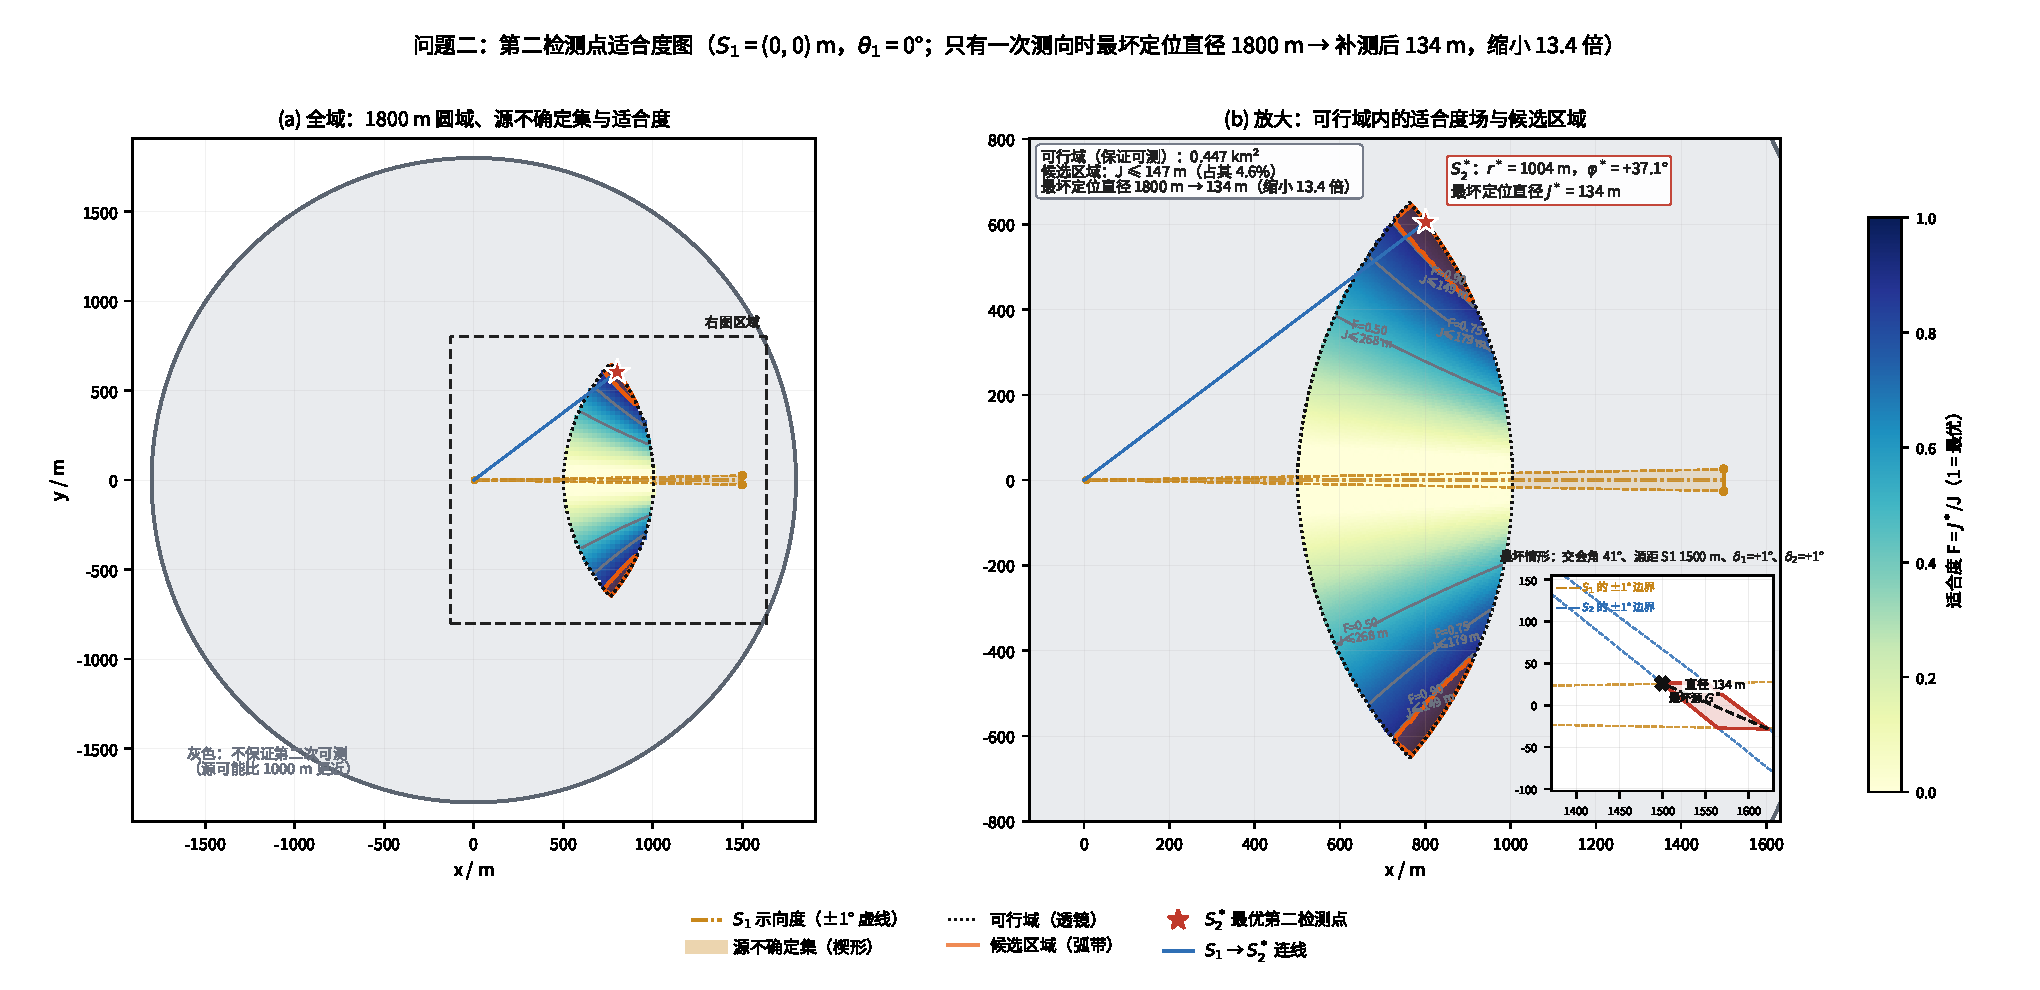
\includegraphics[width=0.98\textwidth]{../figures/t2_suitability.pdf}
  \caption{最优第二检测点与周边区域的适合度场（全域、放大与最坏情形内嵌视图）。}
  \label{fig:suit}
\end{figure}

\subsection{文献判据的对照}

图~\ref{fig:criteria} 把 §\ref{sec:lit} 的四种口径画在一起。左图固定本模型最坏情形的距离
组合（$R_1=1500$ m、$R_2=907$ m），横轴为交会角 $\gamma$，纵轴为定位区域半径（对数坐标）：
精确构造、本文集员闭式、文献 GDOP、文献 CRLB 主半轴与文献几何稀释式五条曲线。可以看到
（i）五条曲线\textbf{走向一致}，都以 $1/\sin\gamma$ 为主导，$\gamma$ 从 $90^\circ$ 降到
$20^\circ$ 时半径放大 $5$ 倍以上；（ii）文献三条曲线明显低于精确构造曲线（约三成），
与表~\ref{tab:criteria} 的数值一致；（iii）本文闭式紧贴精确构造"同口径近似"，在这段
$\gamma$ 区间偏差不到 $10\%$。右图是可行域内 $1276$ 个采样点上"文献 GDOP 判据—本文精确
直径"的双对数散点，点云紧贴对角线（Spearman 秩相关 $0.998$），并标出三个口径各自的最优点。

\begin{figure}[H]
  \centering
  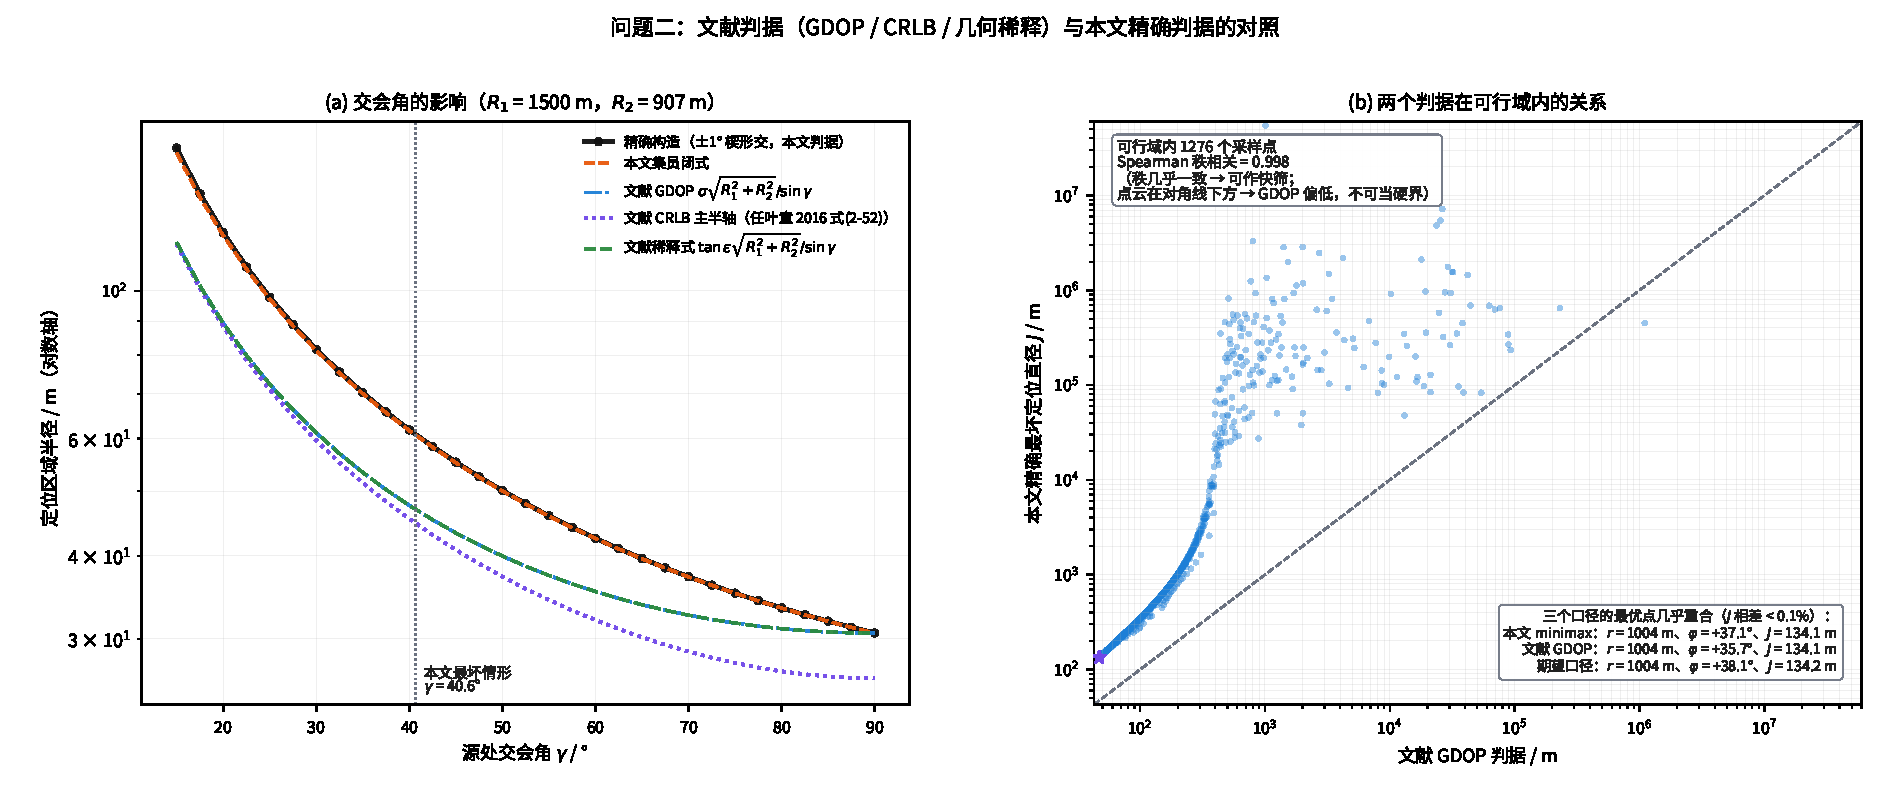
\includegraphics[width=0.98\textwidth]{../figures/t2_criteria.pdf}
  \caption{文献判据与本文判据的对照：(a) 交会角对定位半径的影响；(b) 判据一致性散点。}
  \label{fig:criteria}
\end{figure}

\subsection{准则对照：结论对判据的选择不敏感}

为了回答"换一个判据会不会换一个答案"，本文在完全相同的模型与数据上用三种准则各求一次最
优点，结果列于表~\ref{tab:three}。三个最优点相距不到 $20$ m，最坏直径相差不超过 $0.08\%$，
期望直径相差不超过 $0.2\%$：\textbf{无论按最坏情况、按文献 GDOP 判据、还是按文献常用的期望
精度口径选点，落点都是可行域外缘 $r\approx1004$ m、偏示向度 $36^\circ\sim38^\circ$}。
本文最终采用 minimax 口径，因为清除判据是 $20$ m 硬阈值——需要的是"保证"，不是"平均"。

\begin{table}[H]
  \centering
  \caption{三种准则下的最优点对照（三者都以同一套精确构造与 $1395$ 组合计算）}
  \label{tab:three}
  \small
  \setlength{\tabcolsep}{4pt}
  \begin{tabular}{lccccc}
    \toprule
    \textbf{准则} & $(x,y)$ / m & $r$ / m & $\varphi$ & \textbf{最坏直径 / m} & \textbf{期望直径 / m} \\
    \midrule
    minimax（本文，采用）           & $(801,\;605)$ & $1004$ & $+37.1^\circ$ & $\mathbf{134.08}$ & $56.07$ \\
    文献 GDOP 判据               & $(815,\;586)$ & $1004$ & $+35.7^\circ$ & $134.15$（$+0.05\%$） & $56.18$ \\
    期望精度（Chen 等~\cite{chen2009}）& $(790,\;619)$ & $1004$ & $+38.1^\circ$ & $134.19$（$+0.08\%$） & $\mathbf{56.05}$ \\
    \bottomrule
  \end{tabular}
\end{table}

\subsection{策略的解释}

综合以上结果，第二个检测点的选择策略可以写成三条可以直接执行的规则：

\begin{enumerate}
  \item \textbf{尽量把基线拉长。} 基线越长，源处交会角越大，$1/\sin\gamma$ 越小；但基线受
        可测性限制：源到第二点的距离必须 $\le1000$ m，而源最远可达 $1500$ m，几何上给出
        基线上限 $1005$ m。最优解恰好取在 $1004$ m 处。
  \item \textbf{同时把第二点偏离示向度约 $37^\circ$。} 只拉长基线而方向不变会退化为共线
        （$\gamma\to0$），定位反而变差；偏 $37^\circ$ 既保证"对最远源的交会角最大"，
        又让"对最近源的交会角仍足够大"。
  \item \textbf{两条镜像解等价，任选其一。} 结果关于示向度方向严格镜像对称，现场按障碍与
        路径择优即可。
\end{enumerate}

两个约束同时顶到边界，把最坏交会角锁在约 $41^\circ$——这正是最优点所在处
（若只有基线约束，理论上限是 $\arcsin(1005/1500)=42.1^\circ$，但那时最远源与第二点的距离
会超过 $1000$ m，只能放弃保证）。

\section{灵敏度分析与稳健性}\label{sec:sens}

\subsection{可测性口径：从"一定听得到"到"可能要多测一次"}

本文采用最保守口径（源到第二点的距离 $\le1000$ m）。若允许第二次测向失败后重跑，把可测性
放宽到接收半径上界 $1500$ m，则可行域从 $0.447$ km$^2$ 扩到 $2.737$ km$^2$，最优最坏直径
从 $134.08$ m 降到 $79.99$ m，最优点外移到 $r=1500$ m、$\varphi=+39.8^\circ$（"贴到最远处"），
候选弧带变成 $r\in[1262,1504]$ m、$\theta_1\pm[29.5^\circ,45.5^\circ]$、面积 $0.0931$ km$^2$。
这说明：\textbf{代价主要在"保证"上，不在"方向"上}——放宽保证能白拿 $40\%$ 的精度，但会带来
"白跑一趟"的风险，本文不采用。

\subsection{第一轮已知距离先验}

若第一轮还能给出距离区间（例如通过信号强度或接收时间给出 $d\le1000$ m 的上限），不确定集
被压短，可行域变为 $1.219$ km$^2$，最优最坏直径直接降到 $53.31$ m（最优点
$(769,639)$ m、$r=1000$ m、$\varphi=+39.7^\circ$），候选弧带 $r\in[842,1004]$ m、
面积 $0.0415$ km$^2$。可见\textbf{距离信息是最值钱的信息}：把"最远可能源从 $1500$ m 缩到
$1000$ m"这一条，就能把最坏定位直径减少六成。

\begin{table}[H]
  \centering
  \caption{三种口径下的最优解与候选区域（其余参数不变）}
  \label{tab:sens}
  \small
  \setlength{\tabcolsep}{5pt}
  \begin{tabular}{lcccccc}
    \toprule
    \textbf{口径} & $S_2^*$ / m & $r^*$ / m & $\varphi^*$ & $J^*$ / m & \textbf{可行域 / km$^2$} & \textbf{提升} \\
    \midrule
    缺省（保证 $\le1000$ m）        & $(801,605)$   & $1004$ & $+37.1^\circ$ & $134.08$ & $0.447$ & $13.4$ 倍 \\
    可测性放宽到 $1500$ m           & $(1153,959)$  & $1500$ & $+39.8^\circ$ & $79.99$  & $2.737$ & $22.5$ 倍 \\
    已知 $d\le1000$ m（距离先验）   & $(769,639)$   & $1000$ & $+39.7^\circ$ & $53.31$  & $1.219$ & $33.8$ 倍 \\
    \bottomrule
  \end{tabular}
\end{table}

\subsection{候选区域阈值}

阈值 $\eta$ 只改变弧带的宽度而不改变最优点：$\eta=10\%$ 时面积 $0.02069$ km$^2$，
$\eta=5\%$ 时 $0.00880$ km$^2$，$\eta=2\%$ 时 $0.00289$ km$^2$（表~\ref{tab:band}）。
即"宽容度"与"可现场选择的范围"之间存在直接的、单调的取舍关系，现场可以按需要的余量挑
阈值。

\subsection{检测点位置与示向度方向}

模型与算法对 $S_1$ 的位置与示向度没有任何特殊依赖。用三组完全不同的设定复算：

\begin{itemize}
  \item $S_1=(200,-300)$ m、$\theta_1=45^\circ$：$J^*=134.10$ m；
  \item $S_1=(1700,0)$ m、$\theta_1=180^\circ$：$J^*=134.10$ m；
  \item $S_1=(-900,900)$ m、$\theta_1=225^\circ$：$J^*=79.34$ m、可行域 $0.383$ km$^2$。
\end{itemize}

前两组与缺省解的 $J^*$ 完全相同（$134.10$ m 与 $134.08$ m 的差别来自 $5$ m 认证网格的步长
自适应，属于数值分辨率），说明结论具有\textbf{平移与旋转不变性}——这符合问题的几何性质：
把整幅构型一起平移旋转，直径不变。第三组之所以更好，是因为该检测点距圆域中心 $1273$ m，
示向度指向圆外，最远的那些源（最不友好的共线构型）被 $1800$ m 圆域裁掉了，不确定集本身变短，
可行域也随之变小。这提示了一个有用的工程推论：\textbf{如果检测点靠近圆域边界、且示向度朝外，
第二个检测点的精度要求会更宽松}。

\subsection{判据选择与快筛稳定性}

§\ref{sec:res} 表~\ref{tab:three} 已说明三种准则的最优点相差不足 $20$ m。判据快筛的稳定性
同样在多组口径下检验：GDOP 与精确直径的排序相关在缺省口径为 $0.998$，在可行域被拉长的
两个放宽口径下分别为 $0.942$（可测性放宽）与 $0.946$（距离先验）。$0.94$ 意味着排序略有
损失，但仍足以把几万个候选压缩到几十个，最终结论一律由精确构造复核给出——快筛只影响
"算多久"，不影响"答案是什么"。

\section{模型校验、评价与推广}\label{sec:eval}

\subsection{模型与程序的自校验}

所有结论都由确定性程序给出，程序在每次运行时自动执行一组互相独立的校验，结果写入结论文件。
表~\ref{tab:checks} 汇总了这些校验：几何构造用两套完全不同的方法互对（解析构造 vs 计算几何库
的精确求交），离散化用加密 $3$ 倍复算，文献闭式用数值特征分解对账，最优解用两条独立搜索
路线互认，对称性用镜像点核对，产物用逐字节比对。

\begin{table}[H]
  \centering
  \caption{自校验清单（每次运行自动执行）}
  \label{tab:checks}
  \begin{tabular}{p{0.52\textwidth}p{0.40\textwidth}}
    \toprule
    \textbf{校验项} & \textbf{结果} \\
    \midrule
    解析构造 vs 精确求交（$400$ 例，有效 $213$ 例） & 最大相对偏差 $1.2\times10^{-14}$ \\
    一阶式 vs 精确构造（$\gamma\in[30^\circ,120^\circ]$，$120$ 例） & 中位 $0.078\%$，$98\%$ 的样本 $<1\%$ \\
    离散化加密 $3$ 倍（$d$、$\delta_1$、$\delta_2$ 各 $3$ 倍）复算 $J^*$ & 相对偏差 $6.4\times10^{-15}$ \\
    最坏情形 vs 问题一精确区域口径 & 相对偏差 $0$ \\
    最坏情形是否被圆域截断 & 未截断，顶点数 $4$ \\
    可行域边界的最坏距离 & $\in[1000.0,1000.0]$ m（全部舍入误差内成立） \\
    候选弧带径向连续性 & 每个方位角均连续，断口 $0$ 处 \\
    镜像对称性（镜像点的代价） & 相对偏差 $\le1\times10^{-14}$ \\
    文献闭式 vs 数值特征分解（$53$ 例） & 最大相对偏差 $1.4\times10^{-12}$ \\
    全局认证（$5$ m 网格快筛 $+$ 精确复核 $+$ 细化） & $J=134.0831$ m，与粗搜解相隔 $8.49$ m（未漏盆地） \\
    确定性（两次运行的六个产物） & 逐字节一致 \\
    \bottomrule
  \end{tabular}
\end{table}

\subsection{模型优点}

本模型的第一个优点是\textbf{保证型}：不假设任何误差分布，"第二次一定听得到"与"最坏定位
直径"都是硬保证，直接对应 $20$ m 清除阈值这种硬判据，不会因为分布假设不成立而失效。第二个
优点是\textbf{可解释}：最优解的结构由两条几何事实完全解释——$1/\sin\gamma$ 主导（交会角越大
越好）与两个约束同时顶到边界（基线不超过 $1005$ m、源到第二点的距离不超过 $1000$ m）——
并有一阶解析式与文献的几何稀释结论互相印证，因此结论可以被现场人员理解与记忆。第三个优点
是\textbf{双重认证}：精确构造路线与"文献判据快筛 $+$ 精确复核"路线彼此独立，结果仅相差
$8.5$ m 且后者略优，消除了"粗网格漏掉更好盆地"这一类网格依赖风险。第四个优点是
\textbf{结论稳健}：minimax、文献 GDOP 与期望精度三种准则给出的最优点相距不足 $20$ m、
最坏直径相差小于 $0.1\%$，说明推荐区域不依赖判据的选择。最后，全部结果\textbf{完全可复现}：
程序无随机数，六个产物两次运行逐字节一致，论文中的每个数字都能由结论与校验文件反向核对。

\subsection{模型局限}

\begin{enumerate}
  \item \textbf{最坏界偏保守。} 有界误差模型必须承担"两个 $\pm1^\circ$ 误差同向叠加"的
        最坏情形，因此定位区域比其他口径大约三成。若工程上允许按统计模型评估风险，可用
        期望口径替代；本文已验证两种口径给出的最优点几乎相同（表~\ref{tab:three}），
        所以保守性对\textbf{选点}的影响很小，对\textbf{报出的精度指标}影响较大。
  \item \textbf{不确定集依赖题设上界。} $d\le1500$ m 来自接收半径上限；若该上界估计偏大，
        可行域会偏小、最坏直径偏大（安全方向）；若第一轮能给出距离先验，结果会显著更好
        （§\ref{sec:sens}）。
  \item \textbf{圆域截断按保守处理。} 代价函数用未截断四边形的直径作为上界。在本文的
        最优点处截断并不发生（已验证），但若检测点靠近圆域边界，算法会略微偏好靠内的解，
        属于安全方向的偏差。
  \item \textbf{未纳入执行代价。} 本问只回答"第二点选在哪里"，不考虑机器狗到达该点的里程、
        耗时与地形；两瓣镜像解在精度上完全等价，实际取舍应由路径成本决定。
  \item \textbf{未利用测向误差的空间相关性。} 题面指出同一位置、同一频道重复测量的误差相同
        （系统误差），这意味着"同一地点反复测量"没有信息增益。本文的选点天然满足"两次测
        向来自不同地点"，与该性质相容，但未进一步把它作为约束显式建模。
\end{enumerate}

\subsection{推广}

本模型的核心结构是"不确定集（集员）$+$ 保证型可测性约束 $+$ 最坏情况定位直径最小化 $+$
适合度场"，它可以推广到若干相邻情形。若已掌握部分距离先验，只需把不确定集的径向上界替换为
先验值，算法与图不需要任何改动（§\ref{sec:sens} 已给出该情形的完整结果）。若需要第三次及
以后的测向，把前两次的楔形交作为新的不确定集、重复同一套流程即可选出下一点，代价函数只需把
单项楔形交换成多项楔形交。对于 TDOA、RSSI 等其他观测体制，同样可以写成"不确定集 $+$ 区域
直径"的形式，文献判据层（Fisher 信息 $/$ CRLB）也都有对应形式，本文"判据对照 $+$ 快筛认证"
的框架可以直接复用。若源在观测期间移动，则把式~\eqref{eq:J} 的 $\max$ 换成沿时间轨迹的
$\max$（鲁棒轨迹优化），模型结构不变。

\subsection{结论}

对本题给定的一次测向结果，第二个检测点应当：

\begin{enumerate}
  \item 选在距第一检测点\textbf{尽可能远}（$1000$ m 量级，几何上限 $1005$ m）且相对示向度
        方向\textbf{偏向约 $37^\circ$} 的位置，最优解为
        $S_2^*=(801,605)$ m（$r^*=1004$ m、$\varphi^*=+37.1^\circ$，镜像解等价）；
  \item 该点的最坏定位直径为 $134.08$ m，相比只做一次测向的 $1800$ m 缩小 $13.4$ 倍，
        意味着在最坏情况下也能满足 $20$ m 清除阈值所需的定位收敛要求（配合后续补测）；
  \item 若需要现场灵活性，可在两条镜像弧带中选择：
        $r\in[947.6,1004.5]$ m、$\varphi\in\theta_1\pm[25^\circ,40^\circ]$，
        合计 $0.02069$ km$^2$，其中每一点的适合度都可用 $F=J^*/J$ 或图~\ref{fig:suit}
        的等值线直接读出；
  \item 该结论对判据选择（最坏 $/$ 文献 GDOP $/$ 期望）不敏感，对检测点位置与示向度具有
        平移旋转不变性，稳健可靠。
\end{enumerate}


\newpage
\referencescn
\newpage
\appendixcn

\end{document}